\documentclass[10pt,a4paper]{article}
\usepackage[latin1]{inputenc}
\usepackage{amsmath}
\usepackage{amsfonts}
\usepackage{amssymb}
\usepackage{graphicx}
\author{Oscar Cruz Cervantes 18311638}
\title{EV1.6}
\date{24/09/2019}

\begin{document}
\maketitle
\begin{center}
Sistemas electronicos de interfaz
Ing. Mecatronica 4ºB
\end{center}
\begin{center}

\includegraphics{01.png}
\end{center}
\newpage
\section{Tiristores en convertidores de CA/CA}
\begin{center}
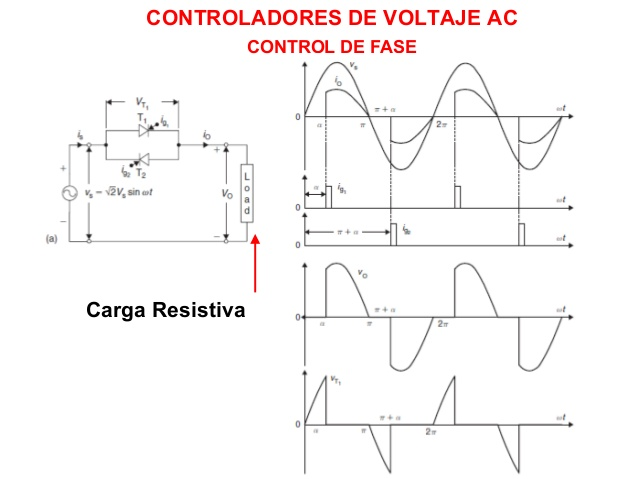
\includegraphics[scale=0.5]{02.jpg}
\end{center}
En los convertidores de CA/CA mediante resistencias se varia el angulo del tirisitor para aumentar o disminuir la potencia del circuito, esto es debido a que los tiristores te permiten rectificar la onda en distintos puntos segun el angulo de la compuerta del tiristor.
\section{Tiristores en convertidores de CD/CA}
\begin{center}
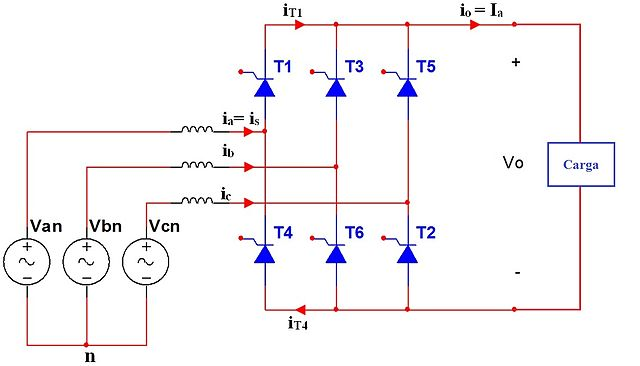
\includegraphics{03.jpg}
\end{center}
En los convertidores de CA/CD los tiristores tienen una funcion similar a la de los diodos, ya que estos rectifiquen la onda, pero en el caso de los tiristores podemos modificar el punto de rectificacion, manteniendo el voltaje en el punto alto de la onda.

\end{document}